%%%%%%%%%%%%%%%%%%%%%%%%%%%%%%%%%%%%%%%%%
% Short Sectioned Assignment
% LaTeX Template
% Version 1.0 (5/5/12)
%
% This template has been downloaded from:
% http://www.LaTeXTemplates.com
%
% Original author:
% Frits Wenneker (http://www.howtotex.com)
%
% License:
% CC BY-NC-SA 3.0 (http://creativecommons.org/licenses/by-nc-sa/3.0/)
%
%%%%%%%%%%%%%%%%%%%%%%%%%%%%%%%%%%%%%%%%%

%----------------------------------------------------------------------------------------
%	PACKAGES AND OTHER DOCUMENT CONFIGURATIONS
%----------------------------------------------------------------------------------------

\documentclass[paper=a4, fontsize=11pt]{scrartcl} % A4 paper and 11pt font size

\usepackage[T1]{fontenc} % Use 8-bit encoding that has 256 glyphs
\usepackage{fourier} % Use the Adobe Utopia font for the document - comment this line to return to the LaTeX default
\usepackage[english]{babel} % English language/hyphenation
\usepackage{amsmath,amsfonts,amsthm} % Math packages

\usepackage{lipsum} % Used for inserting dummy 'Lorem ipsum' text into the template

\usepackage{sectsty} % Allows customizing section commands
\allsectionsfont{\centering \normalfont\scshape} % Make all sections centered, the default font and small caps

\usepackage{fancyhdr} % Custom headers and footers

% use for graph
\usepackage{graphicx} 
\usepackage{subfigure}
\usepackage{caption}
\usepackage{float} 

\pagestyle{fancyplain} % Makes all pages in the document conform to the custom headers and footers
\fancyhead{} % No page header - if you want one, create it in the same way as the footers below
\fancyfoot[L]{} % Empty left footer
\fancyfoot[C]{} % Empty center footer
\fancyfoot[R]{\thepage} % Page numbering for right footer
\renewcommand{\headrulewidth}{0pt} % Remove header underlines
\renewcommand{\footrulewidth}{0pt} % Remove footer underlines
\setlength{\headheight}{13.6pt} % Customize the height of the header

\numberwithin{equation}{section} % Number equations within sections (i.e. 1.1, 1.2, 2.1, 2.2 instead of 1, 2, 3, 4)
\numberwithin{figure}{section} % Number figures within sections (i.e. 1.1, 1.2, 2.1, 2.2 instead of 1, 2, 3, 4)
\numberwithin{table}{section} % Number tables within sections (i.e. 1.1, 1.2, 2.1, 2.2 instead of 1, 2, 3, 4)

\setlength\parindent{0pt} % Removes all indentation from paragraphs - comment this line for an assignment with lots of text

%----------------------------------------------------------------------------------------
%	TITLE SECTION
%----------------------------------------------------------------------------------------

\newcommand{\horrule}[1]{\rule{\linewidth}{#1}} % Create horizontal rule command with 1 argument of height

\title{	
\normalfont \normalsize 
\textsc{University College cork} \\ [25pt] % Your university, school and/or department name(s)
\horrule{0.5pt} \\[0.4cm] % Thin top horizontal rule
\huge The ethical issues in the use of AI in healthcare \\ % The assignment title
\horrule{2pt} \\[0.5cm] % Thick bottom horizontal rule
}

\author{Kai Deng} % Your name

\date{\normalsize\today} % Today's date or a custom date


\begin{document}
\maketitle % Print the title

%----------------------------------------------------------------------------------------
%	PROBLEM 1
%----------------------------------------------------------------------------------------

\section{Introduction}

Based on the improvement of certain theories and the improvement of computer computing power,
AI has achieved rapid development in the 21st century. It raises huge expectaions, has attracted 
significant investment expecialy in Medical and healthcare area (Figure1.1 and Figure1.2). So far, advocates of healthcare AI (HCAI)
have promised the thechnology will improve the accuracy of screening and diagnosis, increase the availability of create
in remote regions and free up physicain's time so that they can engage more with patients \cite{frostPublicViewsEthical2022}.
Meanwhile, questions around the potential exacerbation of health disparities due to modeling biases have raised notable ethical
concerns regarding the use of this technology in healthcare \cite{onianiAdoptingExpandingEthical2023}. Including concerns about privacy and 
data ownership, the risk of harm through biased systems and a lack of human oversight \cite{katiraiEthicsAdvancingArtificial2023}.
Here we are going to disscuess, how did this issues arise and what should we do to solve it.



\begin{figure}[H]
    \centering
    \begin{minipage}[t]{0.48\linewidth}
        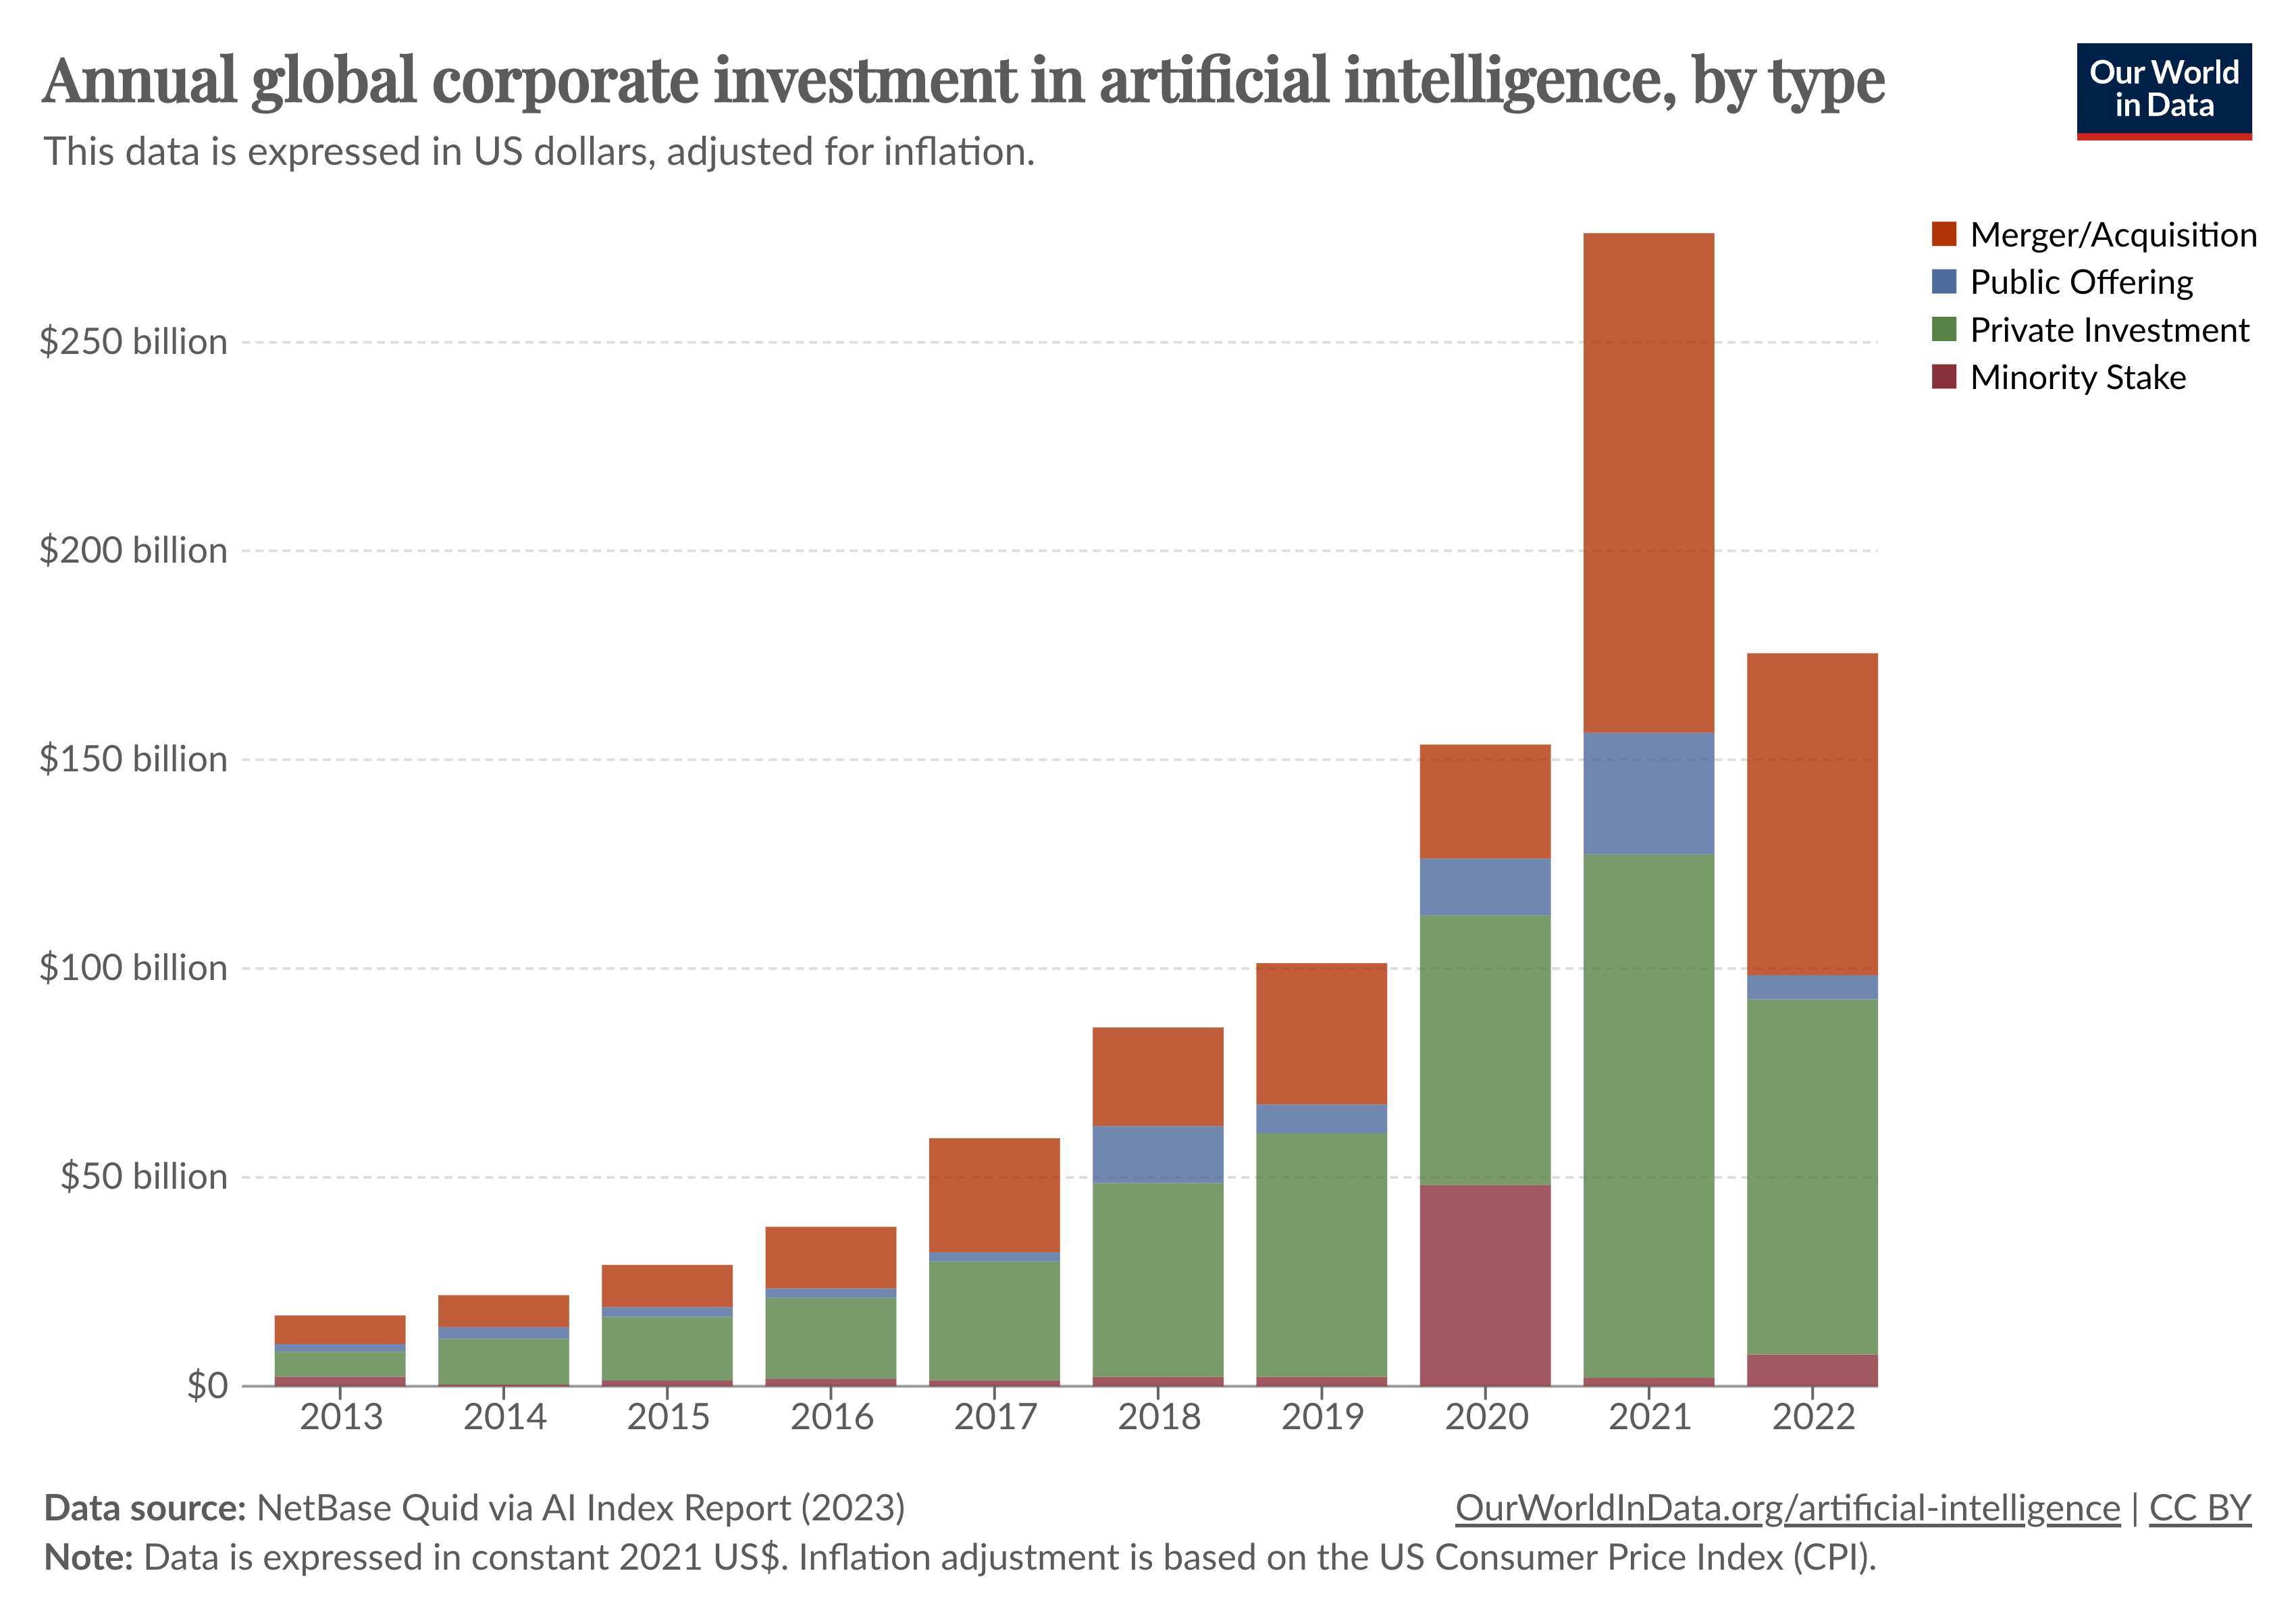
\includegraphics[width=\linewidth]{./data/investment_by_type.png}
        \caption{Annual investment in AI by type}
        \label{fig:investment}
    \end{minipage}\hfill
    \begin{minipage}[t]{0.48\linewidth}
        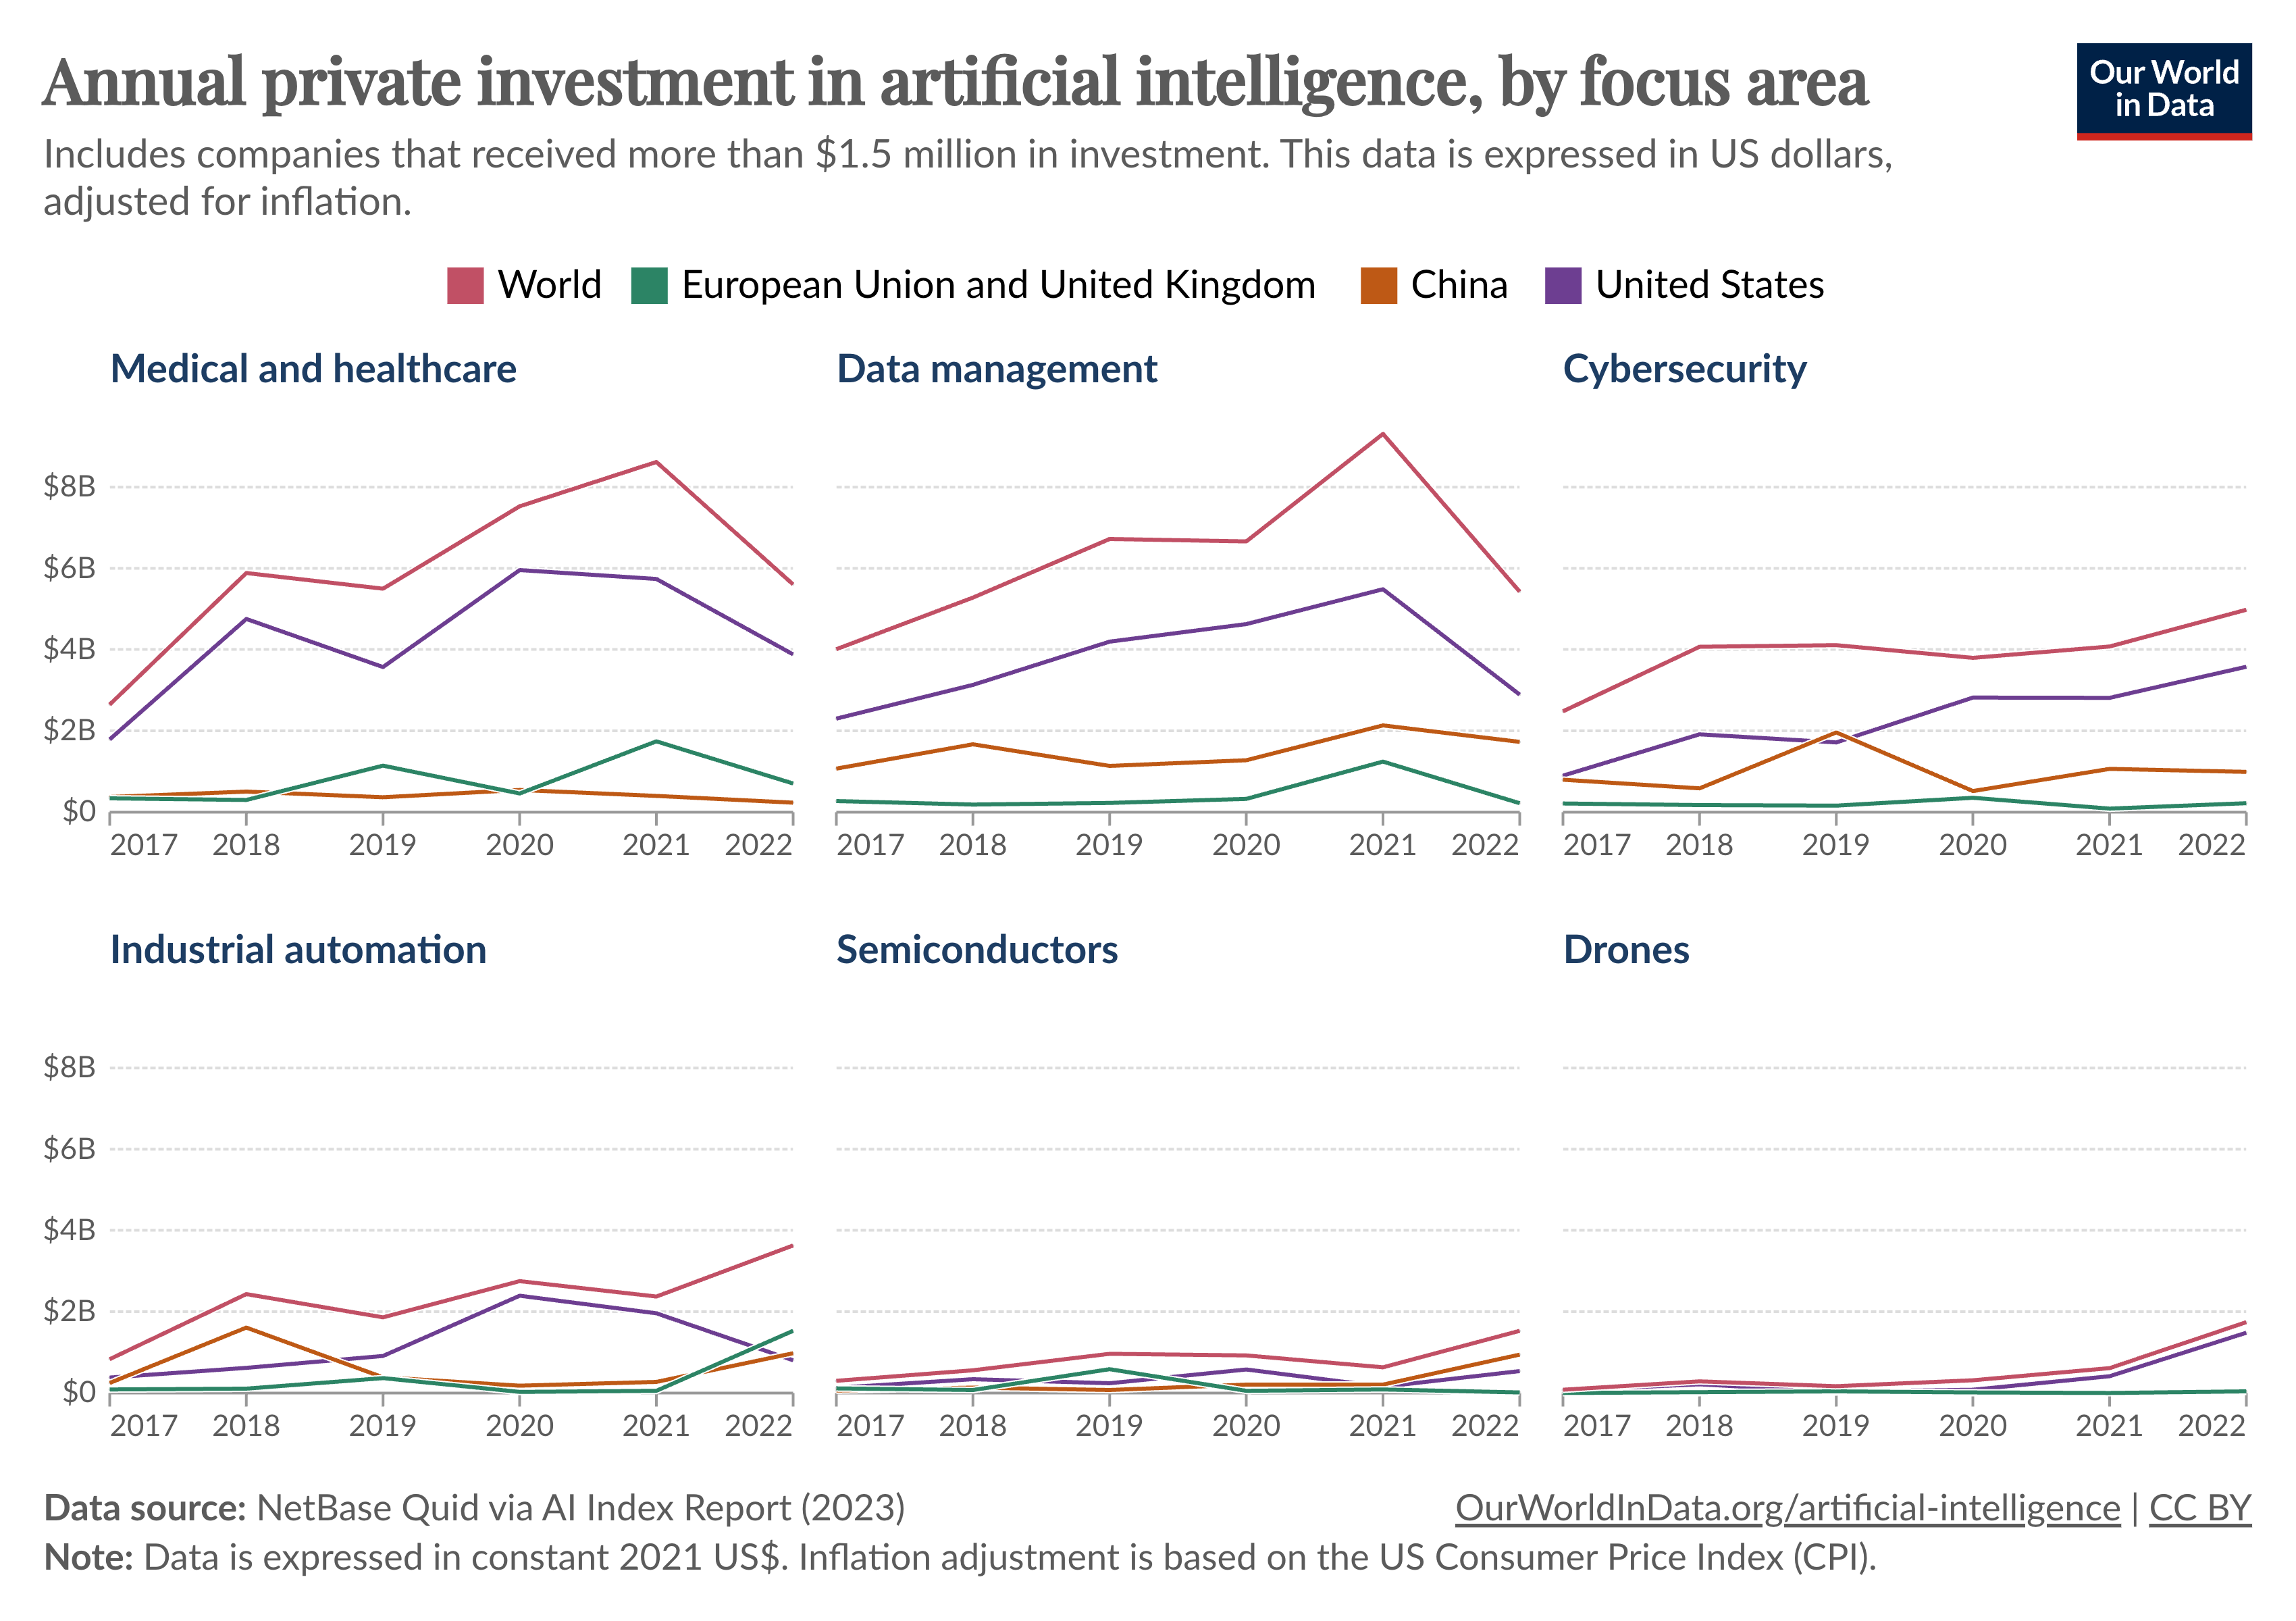
\includegraphics[width=\linewidth]{./data/investment_by_area.png}
        \caption{Annual investment in AI by area}
        \label{fig:views_ai_impact}
    \end{minipage}
\end{figure}


% 大众
\section{section1}
Public may be both benificiaries of new HCAI technologies and the greatest sufferers of AI-related harms. The result highlight that there are still noticeable concerns about 
implementing HCAI in diagnostics and treatment recommendations for patients eith both acute and chronic illnesses, even if these tools are used as a recommendation system under the 
physician experience and wisdom. Individuals may still not be ready to accept and use HCAI \cite{esmaeilzadehPatientsPerceptionsHuman2021}. Patients and publics are important voices In
developing effective and ethical AI governance, but engaging patients and pbulics meanigfully in research about ethical HCAI is challenging. Most people have no first hand experience with HCAI,
and some are unfamiliar with the concept of AI in general, Pulics may have limited understaing of how HCAI may be implemented and limited knowledge about the potential wrongs and harms that coudld
arise from implementing HCAI \cite{frostPublicViewsEthical2022}


\begin{figure}[htbp]
    \centering
    \begin{minipage}[t]{0.48\linewidth}
        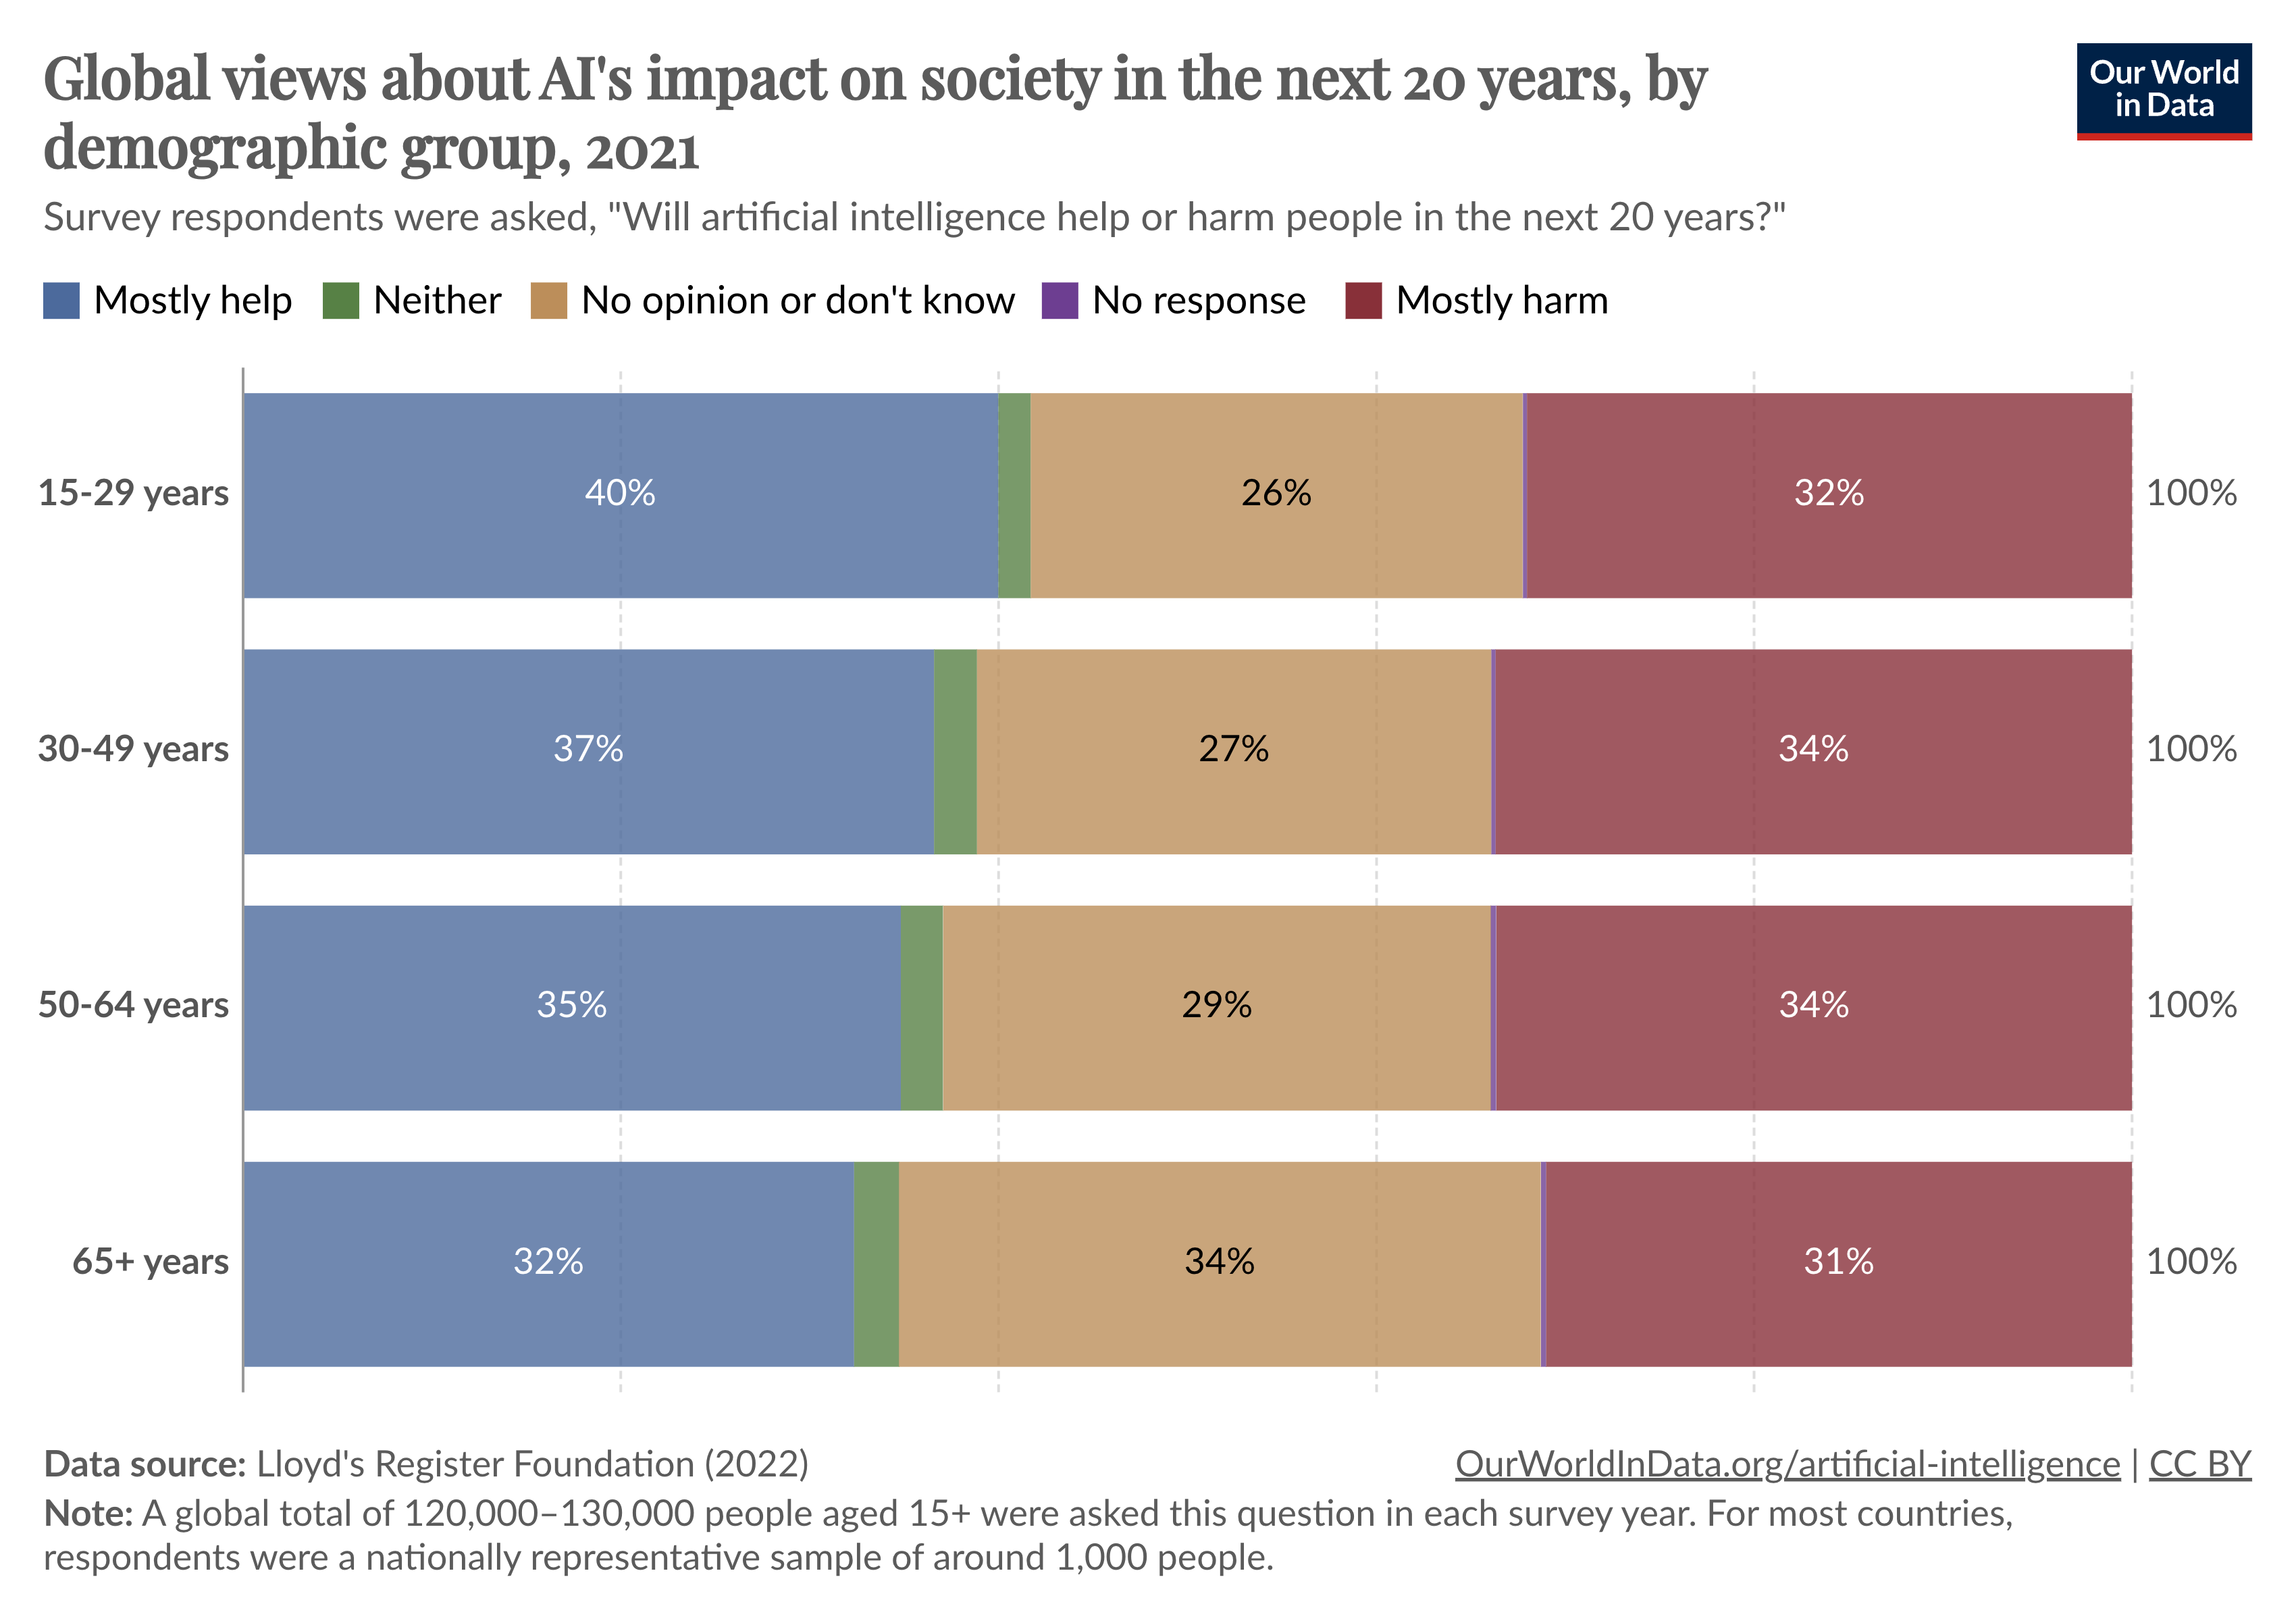
\includegraphics[width=\linewidth]{./data/influence_by_ages.png}
        \caption{Annual private investment in AI}
        \label{fig:investment}
    \end{minipage}\hfill
    \begin{minipage}[t]{0.48\linewidth}
        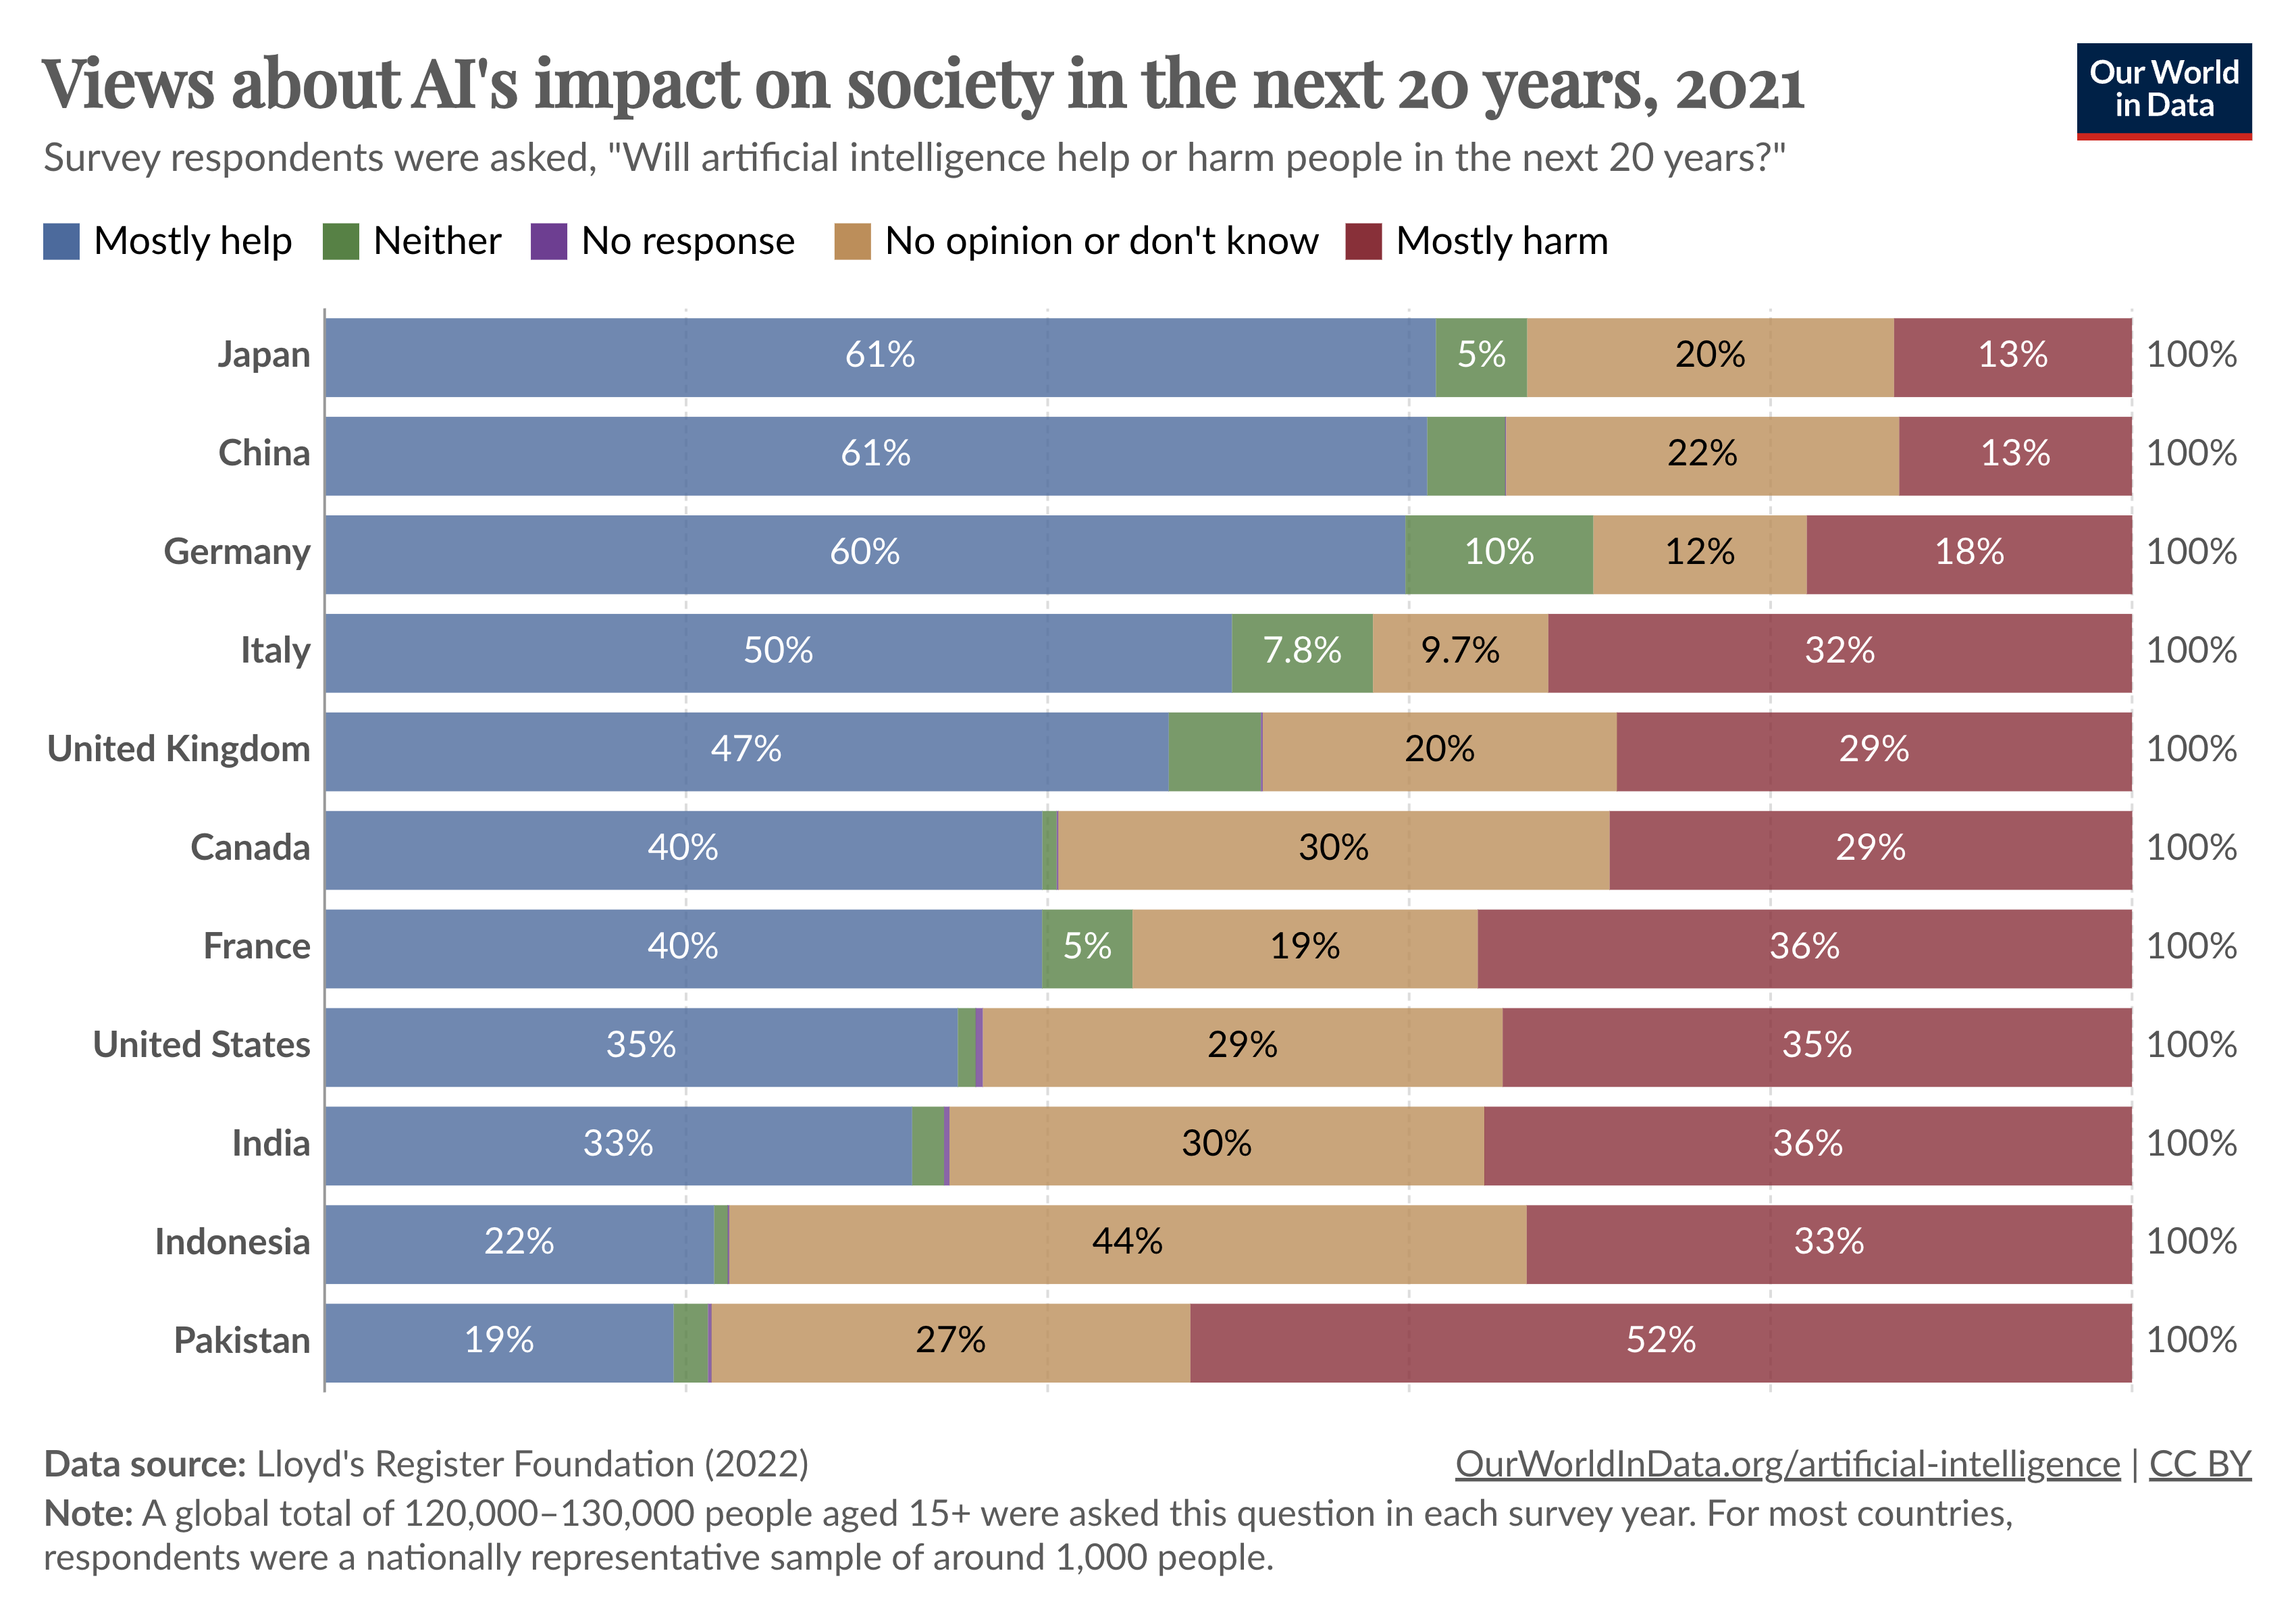
\includegraphics[width=\linewidth]{./data/influence.png}
        \caption{Views on AI's impact on society}
        \label{fig:views_ai_impact}
    \end{minipage}
\end{figure}


% 医生
\section{section2}
Public may be both benificiaries of new HCAI technologies and the greatest sufferers of AI-related harms. The result highlight that there are still noticeable concerns about 
implementing HCAI in diagnostics and treatment recommendations for patients eith both acute and chronic illnesses, even if these tools are used as a recommendation system under the 
physician experience and wisdom. Individuals may still not be ready to accept and use HCAI \cite{esmaeilzadehPatientsPerceptionsHuman2021}. Patients and publics are important voices In
developing effective and ethical AI governance, but engaging patients and pbulics meanigfully in research about ethical HCAI is challenging. Most people have no first hand experience with HCAI,
and some are unfamiliar with the concept of AI in general, Pulics may have limited understaing of how HCAI may be implemented and limited knowledge about the potential wrongs and harms that coudld
arise from implementing HCAI \cite{frostPublicViewsEthical2022}



In general terms it refers to questions involving moral concepts such as right and wrong, or good and bad. 
In most familiar contexts humans intuitively know what is right and wrong, a knowledge of ethics that is acquired during human socialisation.
Sometimes this intuition fails or conflicts with others’ intuitions, at which point ethics appears as a set 
of explicit statements in the form of “you should never / always do X”. Where such statements are not accepted and need justification, 
ethics as a set of philosophical theories is called for. Ethics can be descriptive or normative, abstract or applied. 


% 问题是怎么产生的
% 监管

% 人工智能的制作者


% 处理这个问题的原则
% 人工智能遵循原则和


% 结论

% 人工智能不是洪水猛兽,它在以肉眼可见的速度改变着每一个人的生活方式,它的发展不可阻挡,对于政府来说要加强监管,和对人工智能方面知识的普及
% 对于医生
AI and advanced digital technologies are set to transform healthcare and healthcare systems in a significant way in the twenty-first century




% \begin{figure}[h]
%     \centering
%     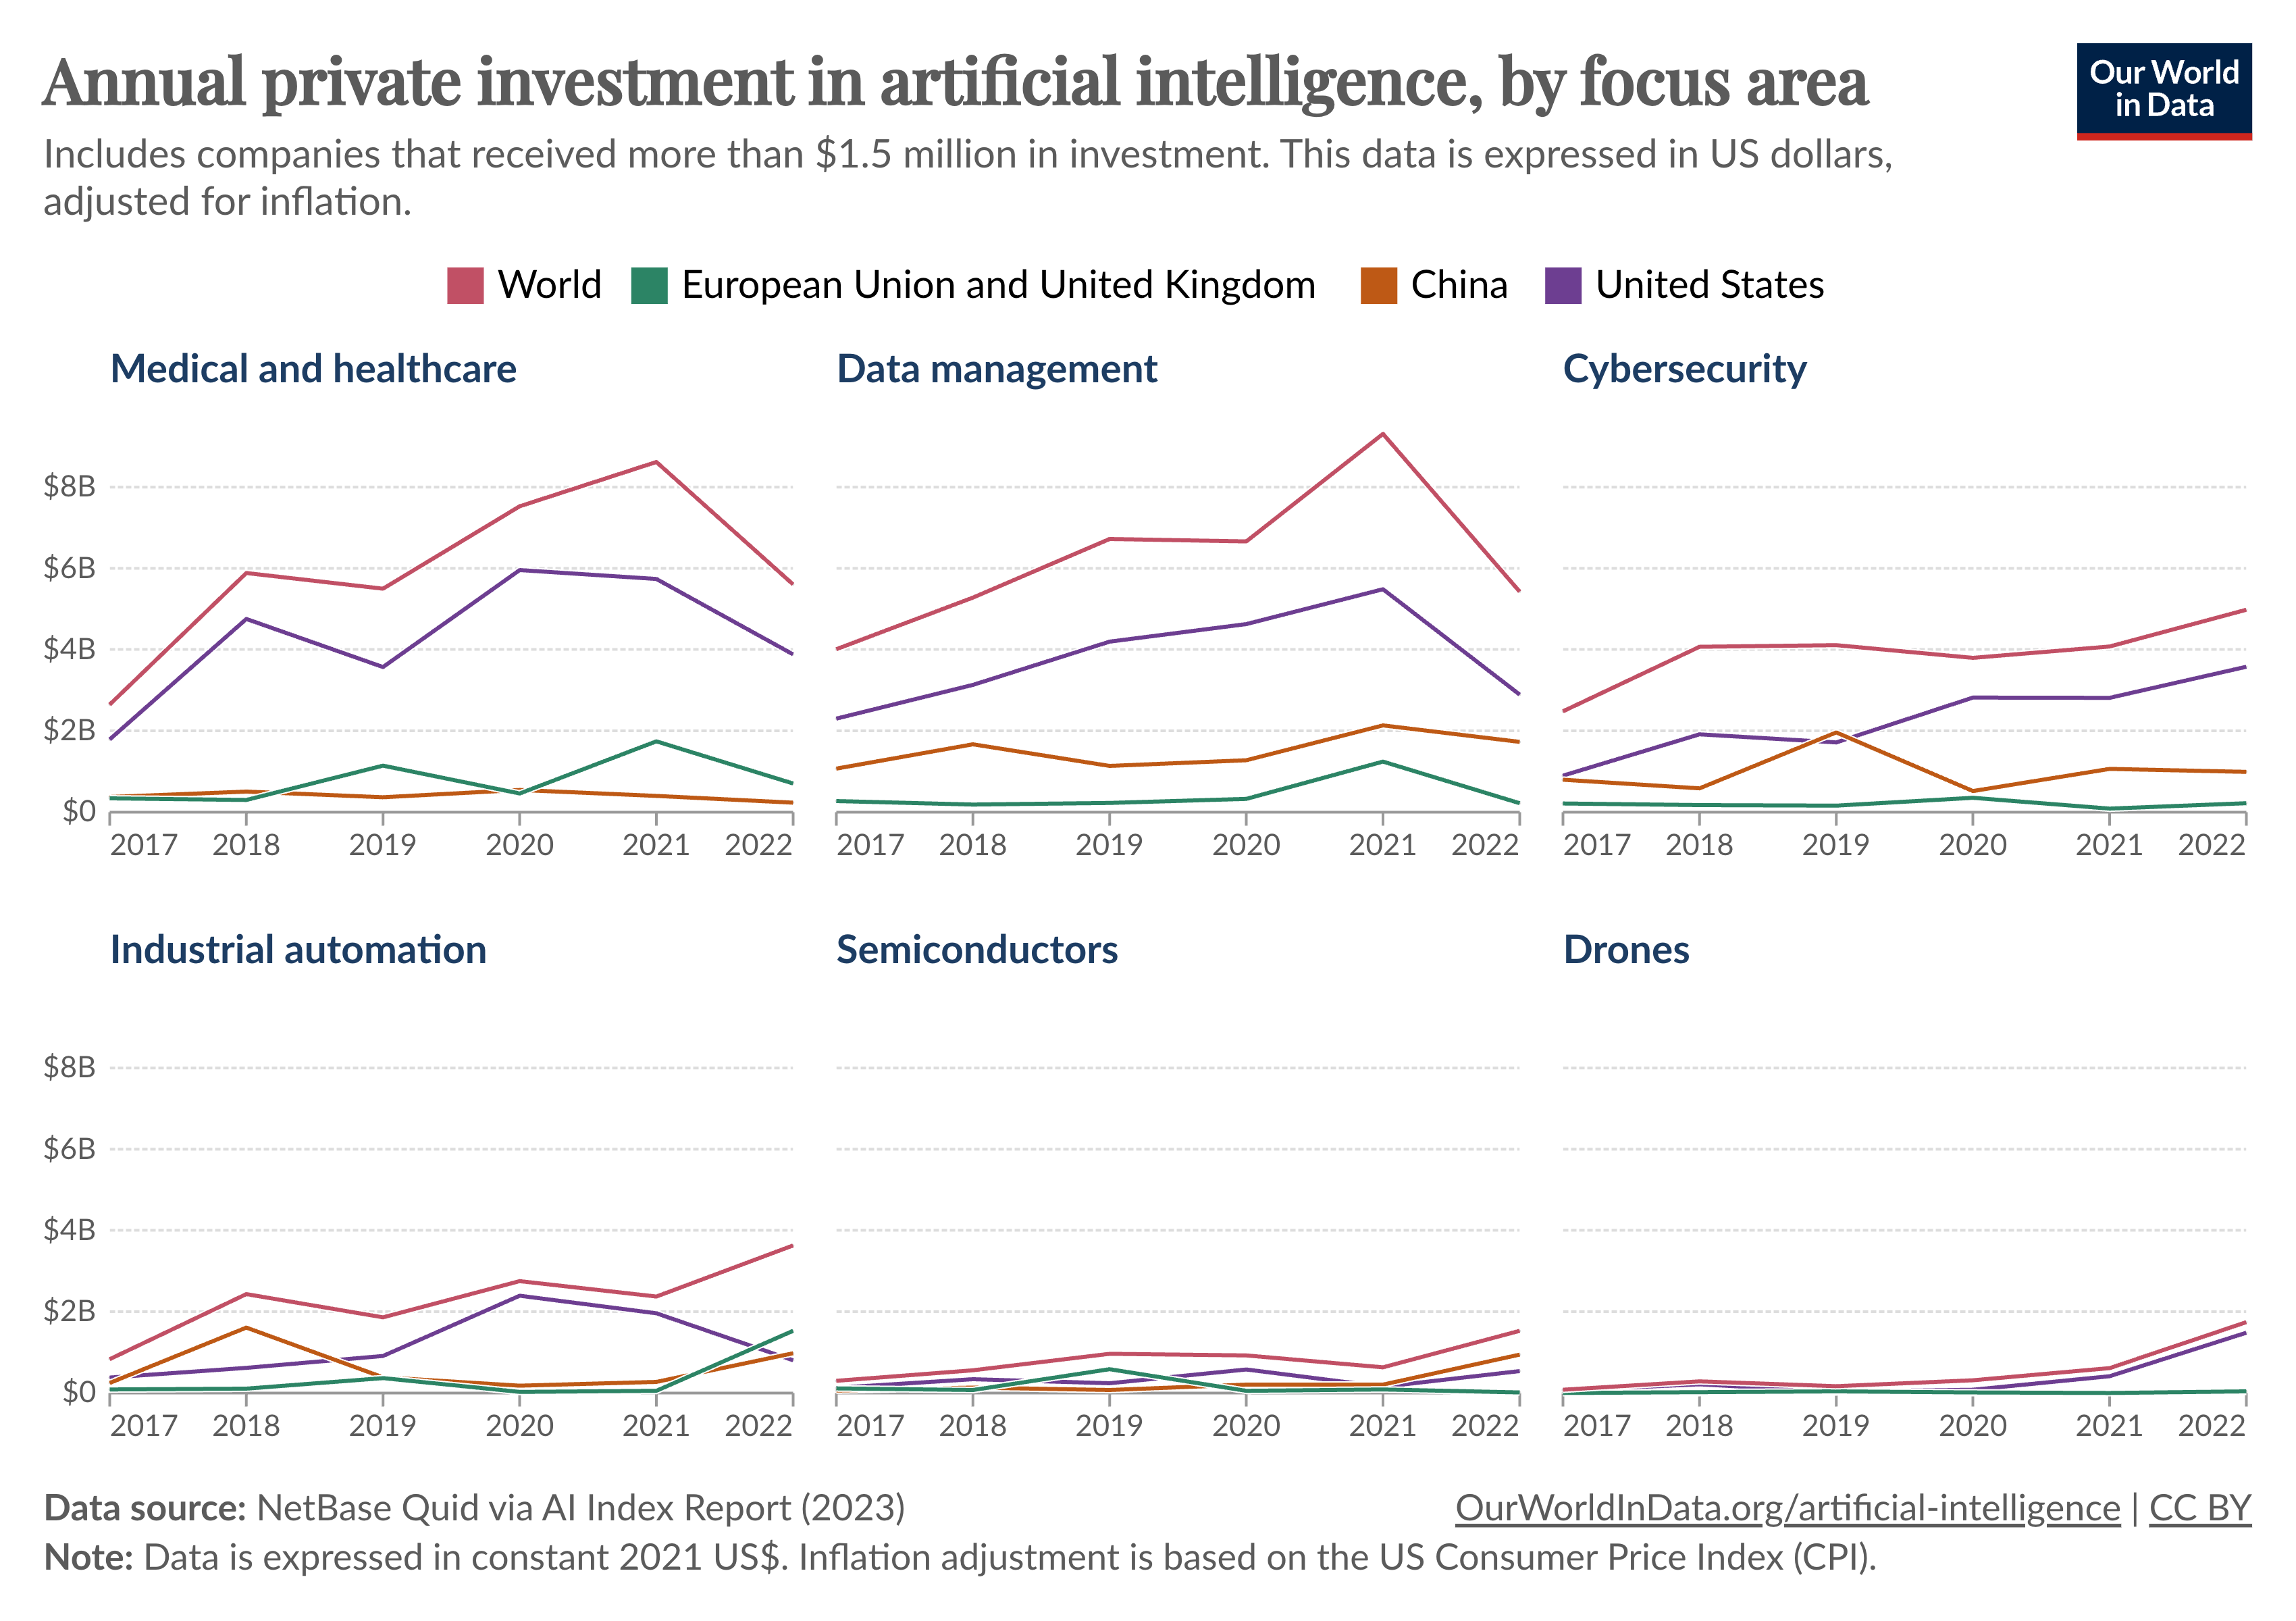
\includegraphics[width=0.9\textwidth]{./data/investegatement.png}
%     \caption{This is the title}
%     \label{fig:my_picture}
% \end{figure}



% \begin{figure}[h]
%     \centering
%     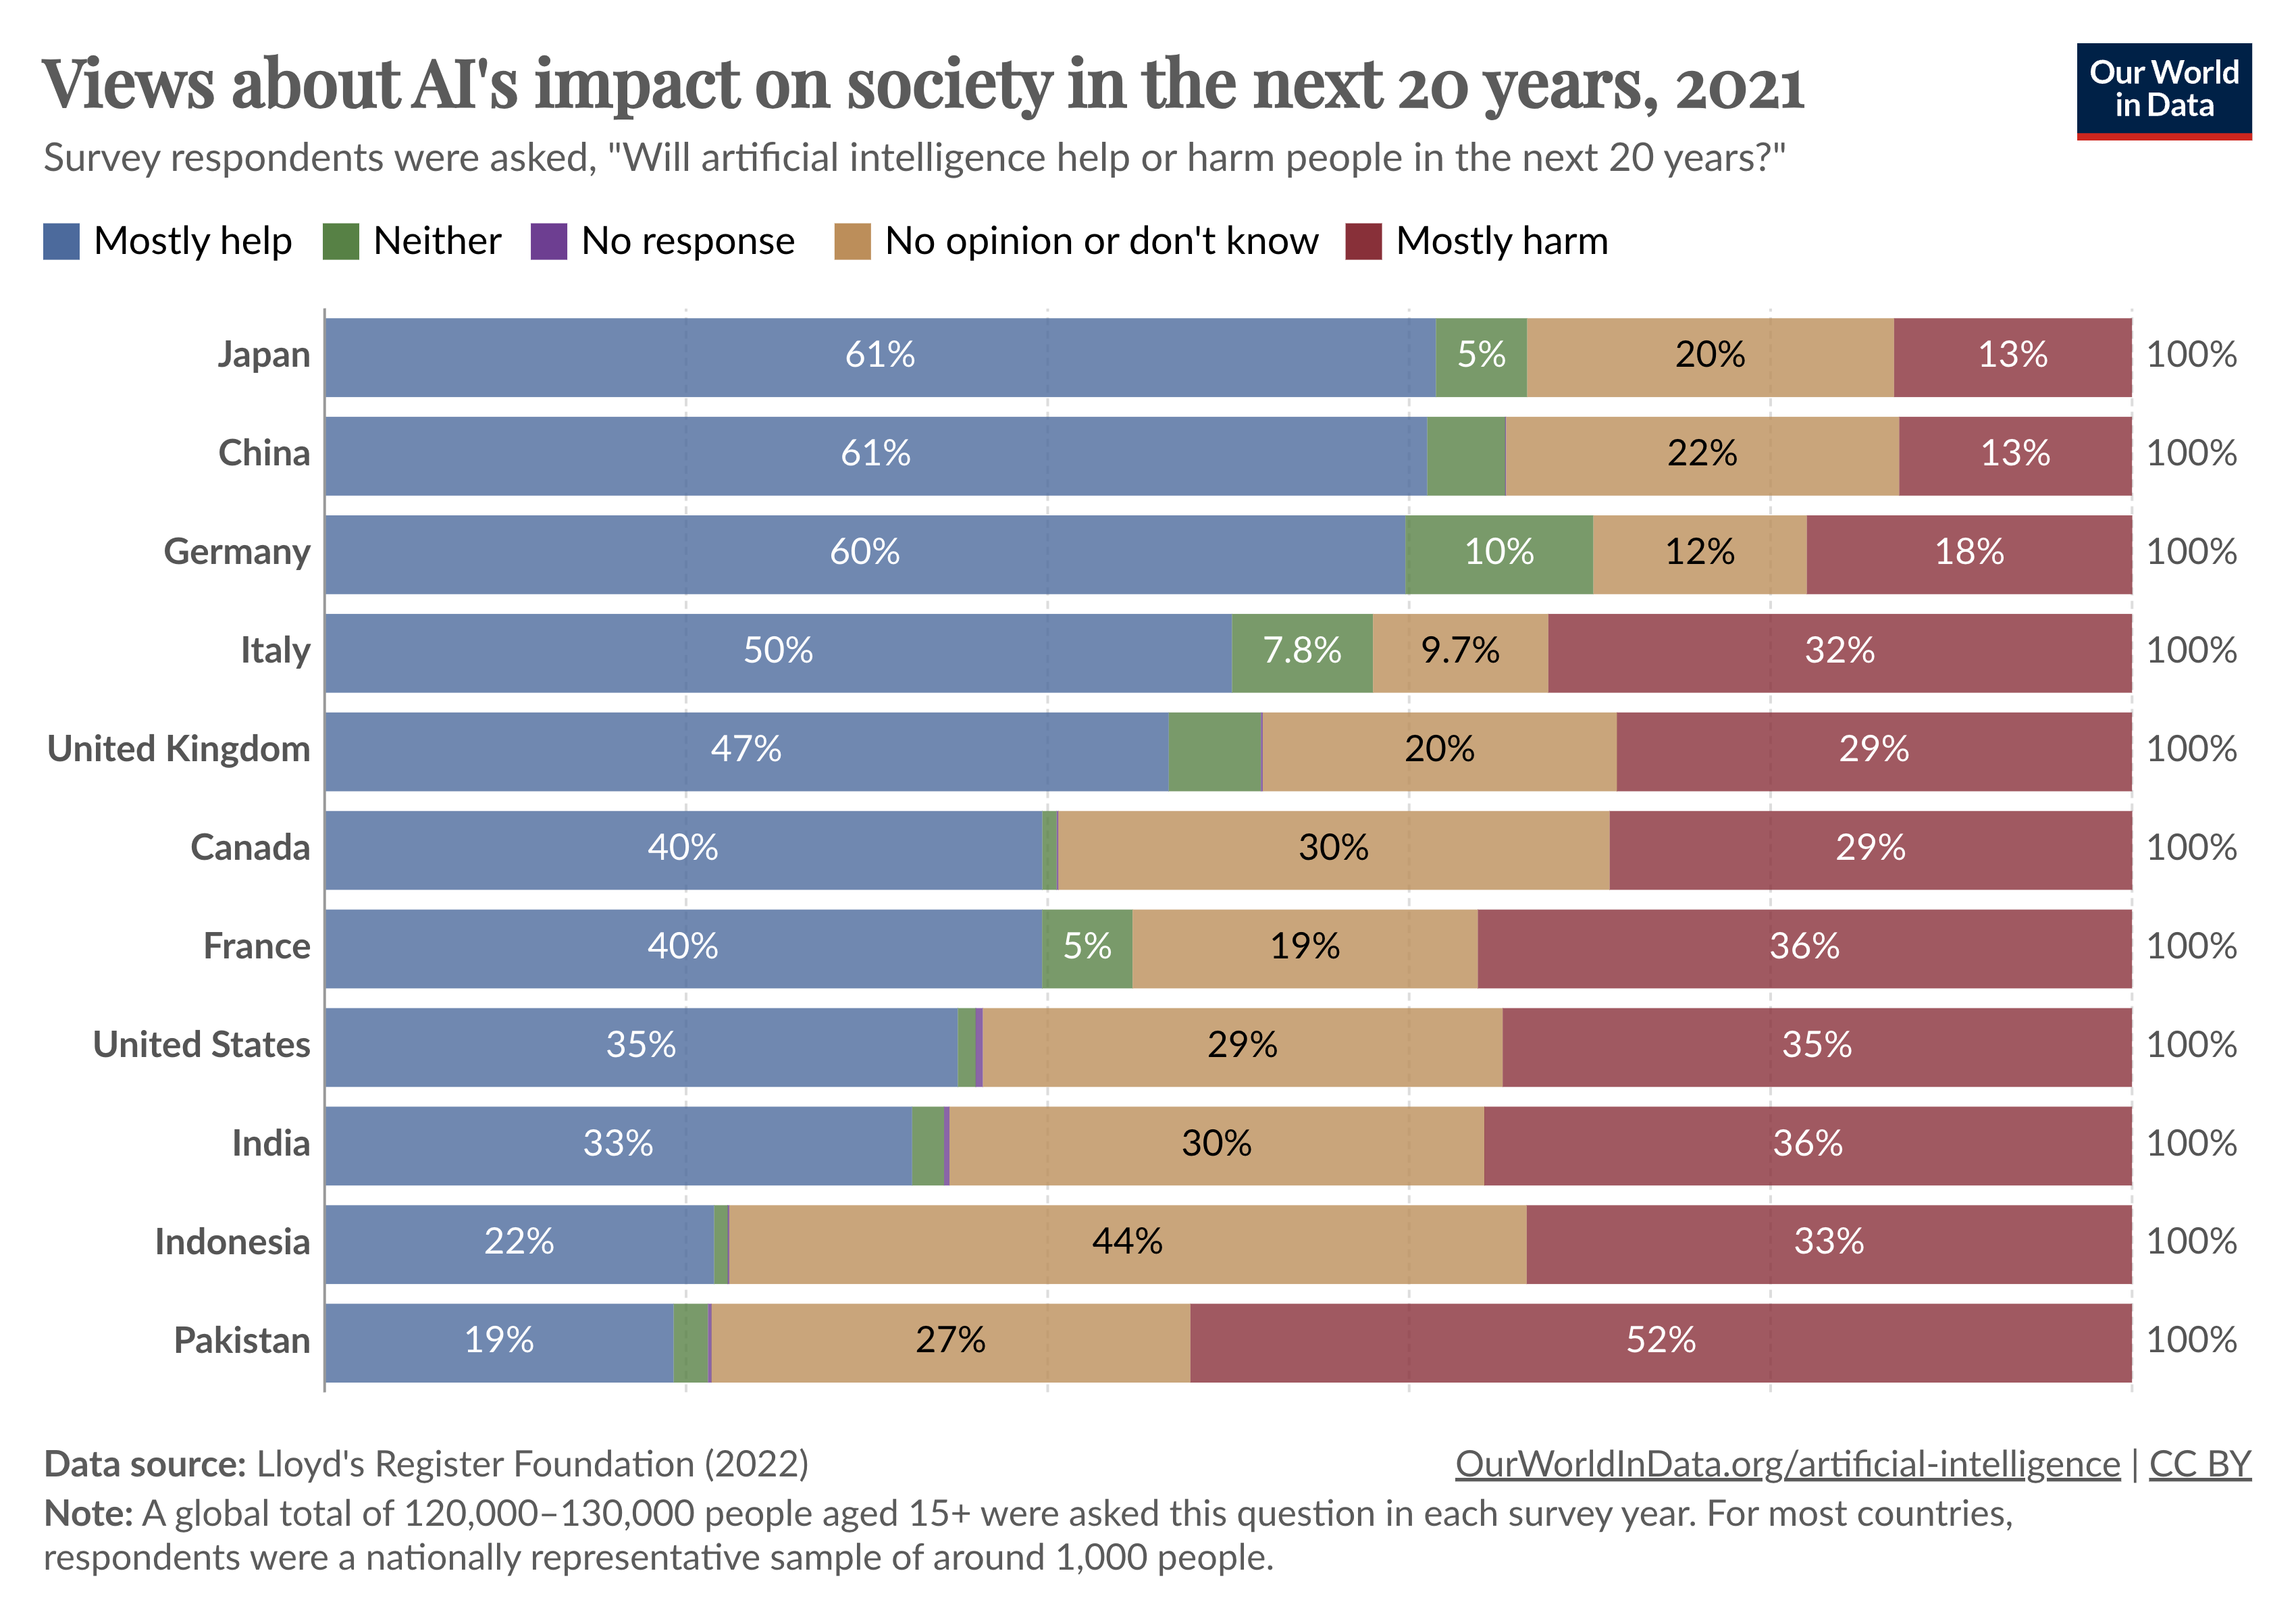
\includegraphics[width=0.9\textwidth]{./data/influence.png}
%     \caption{This is the title}
%     \label{fig:my_picture}
% \end{figure}
















%----------------------------------------------------------------------------------------

\bibliographystyle{unsrt} % This specifies the style of the bibliography
\bibliography{/Users/dengkai/workspace/papers/latex/config/ref} % This should match the name of your .bib file without the extension


\end{document}

